\chapter{Subordinate Shifts}\label{chapter:subordinate}

Given a shift space $Z\subseteq\{0,1\}^G$ one can define its so-called \emph{subordinate shift} $\subord{Z}\subseteq\{0,1\}^G$ by saying that $x\in \subord{Z}$ if and only if there exists a point $z$ in $Z$ such that $x$ is obtained by replacing some $1$'s with $0$'s in $z$ (or in other words $x\leq z$ coordinate-wise). This notion was defined and studied for the shift space $\{0,1,\ldots,n\}^\N$ in ~\cite{KKL18}.

It is worth noting that even if $Z$ is simple, its subordinate shift may be complicated, for example take $Z=\{1^G\}$, then $\subord{Z}=\{0,1\}^G$.
%
However, what turns out, is that computing the entropy of a subordinate shift $\subord{Z}$ under the assumption that $\htop(Z)=0$ is much easier than computing the entropy in general.
%
In Theorem \ref{thm:entropy-density} we prove that if $\htop(Z)=0$, the entropy of $\subord{Z}$ coincides with the ``asymptotic density of ones'' in $Z$.
%
This means that by constructing a space $Z$ with zero entropy and a particular density of $1$'s in $Z$, we can obtain a space $\subord{Z}$ having that given entropy.


 Theorem \ref{thm:entropy-density} plays a crucial role in the proof of Theorem \ref{thm:KriegerProximal}, where the existence of a proximal dynamical system with a given entropy, boils down to a construction of a zero-entropy configuration with a given density of $1$'s.
 %
 Additionally, Theorem \ref{thm:entropy-density} paves a new way for computing the entropy of subordinate shifts: in Lemma \ref{lem:subordinate_measure} we prove that for $Z$ with $\htop(Z)=0$, we have that $\htop(\subord{Z})$ is equal to the maximum (over all $G$-invariant measures) of the measure of the cylinder\footnote{Recall that $[1]_e=\{x\in\{0,1\}^G:x(e)=1\}$ (see Definition \ref{def:cylinder}).} $[1]_e$. 
%

\section{Transitivity of Subordinate Shifts}
In this section we give a characterization of a family of shifts such that their subordinate shifts are transitive. We also introduce some basic properties of the operation of taking subordinate set .

\begin{defn}[Subordinate shift]
For a set $U\subseteq \{0,1\}^G$ we define its {\bf subordinate set} as
\[
\subord{U}\defeq\inbrace{z\in\{0,1\}^G: \exists x\in U~~z\leq x },
\]
where $x\leq z$ means that $x(g)\leq z(g)$ for every $g\in G$.
In particular, if $Z\subseteq \{0,1\}^G$ is a subshift, then we say that $\subord{Z}$ is its {\bf subordinate shift}.
\end{defn}

\noindent
The aim of this section is to prove the following.

\begin{lem}[Transitivity of subordinate shifts]\label{lem:subord-transit2}
Let $x\in X$ and let $\{F_n\}_{n\in\N}$ be a \Folner sequence in $G$. Denote  $Z=\closure{Gx}$. If for every $n\in\N$ there exist infinitely many elements $g\in G$ such that $x_{F_n}\leq x_{F_ng}$, then there exists $z\in\subord{Z}$ such that $z\leq x$ and $\closure{Gz}=\subord{Z}$. 
\end{lem}

\noindent
Before we proceed with the proof, we explain that the word ``shift'' in the name ``subordinate shift'' is indeed justified.
\begin{lem}\label{lem:subordinate_shift}
If $Z\subseteq\{0,1\}^G$ is a subshift, then its subordinate shift $\subord{Z}$ is also a subshift in $\{0,1\}^G$ (i.e., it is closed and invariant).
\end{lem}

\begin{proof}
Clearly, $\subord{Z}$ is $G$-invariant. We show that it is closed. Let $\{x^{(n)}\}_{n\in\N}\subseteq \subord{Z}$ converge to some $x\in\{0,1\}^G$. Then there exists $\{z^{(n)}\}_{n\in\N}\subseteq Z$ such that $x^{(n)}(g)\leq z^{(n)}(g)$ for every $n\in\N$ and $g\in G$. Since $Z$ is compact, there exists a subsequence $\{z^{(k_n)}\}_{n\in\N}$ that converges to some element $z\in Z$. For simplicity assume that $k_n=n$ for every $n\in\N$. We show that $x(g)\leq z(g)$ for every $g\in G$. Fix $g\in G$. If $z(g)=0$, then there exists $N\in\N$ such that for $n>N$ we have $z^{(n)}(g)=0$. Therefore $x^{(n)}(g)=0$ for $n>N$, which implies $x(g)=0$.
\end{proof}

\noindent
Next, we show how operations of taking a subordinate set and a closure of a set interact with each other.
\begin{lem}\label{lem:subord-closure-comute}
The closure of a set commutes with the operation of taking its subordinate set, that is, for every $U\subseteq \{0,1\}^G$ we have $\subord{\closure{ U}}=\closure{\subord{ U}}$.
\end{lem}

\begin{proof}
Clearly, $\subord{U}\subseteq \subord{\closure{ U}}$. Thus, since $\subord{\closure{ U}}$ is closed (by Lemma \ref{lem:subordinate_shift}), we have $\closure{\subord{ U}}\subseteq \subord{\closure{ U}}$. 
%
Next, we justify the converse inclusion. Fix a \Folner sequence $\{F_n\}_{n\in\N}$. Let $x\in \subord{\closure{ U}}$. Then there exists $y\in\closure U$ such that $x\leq y$. We can find $\{y_n\}_{n\in\N}\subseteq U$ such that $y_n\to y$ as $n\to\infty$. Passing to a subsequence if necessary, we can assume that $x_{F_n}\leq (y_n)_{F_n}$ for every $n\in\N$. Now, for every $n\in \N$ define $x_n\in\{0,1\}^G$ as follows: 
\[
(x_n)_{F_n}=x_{F_n}~~~~~~\mbox{ and }~~~~~~ (x_n)_{G\setminus F_n}\equiv 0.
\]
Then, certainly, $x_n\to x$ as $n\to\infty$. Moreover,  for every $n\in\N$ we have $x_n\leq y_n$, thus $x_n\in\subord{U}$. Hence $x\in \closure{\subord{ U}}$.
\end{proof}

\noindent
We need one more technical lemma to prove Lemma \ref{lem:subord-transit2}.

\begin{lem}\label{lem:subord-transit1}
Let $x\in X$ and let $\{F_n\}_{n\in\N}$ be a \Folner sequence in $G$. If $z\in\subord{\closure{Gx}}$ is such that for every $n\in\N$ and for every $w\in\{0,1\}^{F_n}$ satisfying $w\leq x_{F_n}$ there exists $g\in G$ such that $z_{F_ng}=w$, then $\closure{Gz}=\subord{\closure{Gx}}$.
\end{lem}

\begin{proof}
Denote $Z=\closure{Gx}$.
Since $z\in\subord{Z}$, it is clear that ${Gz}\subseteq \subord{Z}$. But $\subord{Z}$ is closed (by Lemma\ref {lem:subordinate_shift}), hence we also have $\closure{{Gz}}\subseteq \subord{Z}$. Now, we prove the converse inclusion. By Lemma \ref{lem:subord-closure-comute} we have $\subord{Z}=\closure{\subord{Gx}}$. Thus, since $\closure{Gz}$ is closed, it is enough to show that $\subord{Gx}\subseteq \closure{Gz}$. Fix $y\in \subord{Gx}$. Then there exists $g\in G$ such that $y\leq gx$, which implies $g^{-1}y\leq x$. This in particular means that $(g^{-1}y)_{F_n}\leq x_{F_n}$ for every $n\in\N$. Therefore $g^{-1}y\in\closure{Gz}$, and thus $y\in\closure{Gz}$.
\end{proof}


\begin{proof}[Proof of Lemma \ref{lem:subord-transit2}]
Denote $Z= \closure{Gx}$ and recall that
\[
\subord{Z} = \{y\in\{0,1\}^G:\exists z\in Z \,\,\,\forall g\in G \,\,\,\, y(g)\leq z(g) \}.
\]
Moreover, for every $n\in\N$ define
\[
W_n\defeq \inbrace{w\in\{0,1\}^{F_n}: w\leq x_{F_n}}
\] 
and denote 
\[
W\defeq \bigcup_{n\in\N} W_n.
\]
Now, let $w_1,w_2,w_3,\ldots$ be an arbitrary enumeration of $W$, further for every $k\in\N$ denote by $n_k$ the unique index such that $w_k\in W_{n_k}$. 

If we construct an element $z\in\subord Z$ such that for every $k\in\N$ the following holds:
\[
\mbox{\Prop{k}:  there exists $g_k\in G$ such that $z_{F_{n_kg_k}} = w_k$},
\]
then by Lemma \ref{lem:subord-transit1} we obtain the claim.

We inductively construct non-icreasing sequence of elements $z_k\in\subord{Z}$ and subsequently define $z$ as its limit:
\[
z\defeq\lim_{k\to\infty} z_k. 
\]
Note that the existence of this limit follows from monotonicity of $\{z_k\}_{k\in\N}$.
In the $k$-th step of the construction we define $z_k\in\subord{Z}$ modifying $z_{k-1}$ such that \Prop{k} is satisfied for $z_k$. To assure that this does not break $\Prop{i}$ for any $i<k$, we need to be careful choosing indices in $z_k$ that we modify. Formally, in the $k$-th step we choose $g_k\in G$ and construct $z_k\in\subord{Z}$ such that:
\begin{enumerate}[(1)]
\item\label{eq:z_k_leq_z_k-1} $z_{k}\leq z_{k-1}$,
\item\label{eq:z_k_eq_w_k} $(z_k)_{F_{n_kg_k}}=w_k$,
\item\label{eq:z_k_eq_z_k-1} $(z_k)_{G\setminus F_{n_kg_k}}=(z_{k-1})_{G\setminus F_{n_kg_k}}$
\item\label{eq:empty_intersection_Fg} $F_{n_k}g_k$ is disjoint from $F_{n_i}g_i$ for every $i<k$. 
\end{enumerate}


In the base step of the construction for $k=0$, we set $z_0=x$. In the $k$-th step, having $z_{k-1}\in\subord{Z}$ constructed, we define $z_{k}\in\subord{Z}$ as follows: as $g_k$ we choose an element $g\in G$ such that 
\begin{enumerate}[(i)]
\item\label{eq:x_F_k_leq_x_F_k-1} $x_{F_{n_k}}\leq x_{F_{n_k}g}$,
\item\label{eq:empty_inters_choice} $F_{n_k}g\cap F_{n_i}g_i=\emptyset$ for every $i<k$.
\end{enumerate}
Note that by the assumption about $x$, condition \eqref{eq:x_F_k_leq_x_F_k-1} is satisfied for infinitely many elements $g\in G$. Further, condition \eqref{eq:empty_inters_choice}  holds for all but finitely many $g\in G$. Consequently, there exists $g_k\in G$ that satisfies both these conditions.

Next we define $z_k\in\subord{Z}$ as follows:
\[
(z_k)_{F_{n_k}g_k} \defeq w_k ~~~~~~\mbox{ and } ~~~~~~ (z_k)_{G\setminus F_{n_kg_k}}\defeq(z_{k-1})_{G\setminus F_{n_kg_k}}.
\]
Now, observe that conditions \eqref{eq:z_k_eq_w_k} and \eqref{eq:z_k_eq_z_k-1} follow directly from the definition of $z_k$. Further, condition \eqref{eq:empty_intersection_Fg} follows from \eqref{eq:empty_inters_choice}. Finally, condition \eqref{eq:z_k_leq_z_k-1} holds since $w_k\leq x_{F_{n_k}}\leq x_{F_{n_k}g_k}$.
\end{proof}

\noindent
In the example below we show that it is not true in general that a subordinate of a transitive shift space is transitive.
\begin{example}
Let $x\in\{0,1\}^\Z$ be defined as
\[
x\defeq \ldots 0 0 0 0.11 0 0 0 0 \ldots.
\]
Then $\closure{Gx}=Gx\cup\{0^\Z\}$ and  $\subord{\closure{Gx}}=Gx\cup Gy\cup\{0^\Z\}$, where
\[
y\defeq \ldots  0 0 00.10 000 0 \ldots.
\]
Now, it is clear that $\subord{\closure{Gx}}$ is not transitive, because up to shifts there are only three distinct elements in this space: $x$, $y$ and $0^\Z$, none of which has a dense orbit.
\end{example}

\section{Entropy} 

The main result of this section is to prove that the maximum asymptotic density of ones in a subshift $Z$ coincides with $\htop(\subord{Z})$ provided $\htop(Z)=0$.

\begin{thm}\label{thm:entropy-density}
Let $G$ be a countable amenable group with a \Folner sequence $\{F_n\}_{n\in\N}$. If $Z\subseteq\{0,1\}^G$ is a subshift such that $\htop(Z)=0$, then the entropy of its subordinate shift $\subord{Z}$ is given by 
\[
\htop(\subord{Z})=\log (2)\lim_{n\to\infty}\frac{1}{|F_n|}\max\inbrace{\sum_{g\in F_n} w(g): w\in \mathcal B_{F_n}(Z)}.
\]
\end{thm}

\begin{proof}
Let $\{F_n\}_{n\in\N}$ be a \Folner sequence in $G$. Since $\subord{Z}\subseteq\{0,1\}^G$ is a subshift, we can use the formula from Lemma \ref{lem:subshift_entropy}, that is,
\[
\htop(\subord{Z})=\lim_{n\to\infty}\frac{\log|\lang_{F_n}(\subord{Z})|}{|F_n|},
\]
where $\lang_{F_n}(\subord{Z})$ denotes the collection of all patterns that appear in elements of $\subord{Z}$ over all the translations of $F_n$ (Definition \ref{def:patterns_over_F}).
By the assumption we have
\[
0=\lim_{n\to\infty}\frac{\log|\lang_{F_n}(Z)|}{|F_n|} =\lim_{n\to\infty}\log|\lang_{F_n}(Z)|^{|F_n|^{-1}},  
\]
thus
\[
\lim_{n\to\infty}|\lang_{F_n}(Z)|^{|F_n|^{-1}} =1.
\]
This gives us a bound on the number of patterns appearing in $Z$ over $F_n$ for sufficiently large $n$. Formally, 
for every $\eps>0$ there exists $N\in\N$ such that for every $n\geq N$, we have
\[ 
|\lang_{F_n}(Z)|\leq(1+\eps)^{|F_n|}.
\] 
Therefore 
\begin{equation}\label{eq:BFnGora}
|\lang_{F_n}(\subord Z)|\leq(1+\eps)^{|F_n|}2^{d_n},
\end{equation}
where 
\[
d_n\defeq \max\inbrace{\sum_{g\in F_n} w(g): w\in \mathcal B_{F_n}(Z)}.
\]
Clearly, we also have 
\begin{equation}\label{eq:BFnDol}
|\lang_{F_n}(\subord Z)|\geq2^{d_n},
\end{equation}
Combining inequalities (\ref{eq:BFnGora}) and (\ref{eq:BFnDol}), taking logarithm and dividing by $|F_n|$, we obtain
\[
\frac{d_n}{|F_n|}\log 2 \leq \frac{\log|\lang_{F_n}(\subord Z)|}{|F_n|}\leq \frac{d_n}{|F_n|}\log 2 + \log(1+\eps).
\]
Then, passing to the limit, one has
\[
\limsup_{n\to\infty} \frac{d_n}{|F_n|}\log 2 \leq\lim_{n\to\infty} \frac{\log|\lang_{F_n}(\subord Z)|}{|F_n|}\leq \liminf_{n\to\infty}\frac{d_n}{|F_n|}\log 2 + \log(1+\eps).
\]
Since $\eps$ was arbitrary, we obtain 
\[
\lim_{n\to\infty} \frac{\log|\lang_{F_n}(\subord Z)|}{|F_n|} = \lim_{n\to\infty}\frac{d_n}{|F_n|}\log 2 . \qedhere
\]
%-------------------------------------------------------------------------------------------------------
\end{proof}

\noindent As our next result we prove that the maximum measure of the identity cylinder is equal, roughly, to the asymptotic maximum density of ones in $x$. (Recall that by $[1]_e$ we denote the cylinder $\{x \in \{0,1\}^G: x(e) = 1\}$)

\begin{lem}\label{lem:max_measure_dens_ones}
Let $G$ be a countable amenable group.
If $Z\subseteq\{0,1\}^G$ is a subshift, then
\[
\max_{\mu\in\mathcal{M}_G(Z)}\mu([1]_e) = 
\lim_{n\to\infty}\frac{1}{|F_n|}\max\inbrace{\sum_{g\in F_n} w(g): w\in \mathcal B_{F_n}(Z)}.
\]
\end{lem}

\begin{proof}
First, note that the limit in the right-hand side exists by Lemma \ref{lem:LW}.

Next, fix a subshift $Z\subseteq\{0,1\}^G$ and denote 
\[
d_n\defeq\max\inbrace{\sum_{g\in F_n} w(g): w\in \mathcal B_{F_n}(Z)}.
\]
First we show that 
\[
\lim_{n\to\infty}\frac{d_n}{|F_n|} \geq \max_{\mu\in\mathcal{M}_G(Z)}\mu([1]_e).
\]
In other words, we prove that for every $\mu\in\mathcal{M}_G(Z)$, we have
\[
\alpha\defeq\lim_{n\to\infty}\frac{d_n}{|F_n|} \geq\mu([1]_e).
\]
Assume to the contrary that there exists $\mu\in\mathcal{M}_G(Z)$ and $\eps>0$ such that 
$
\mu([1]_e)=\alpha+\eps.
$
Then, since $\mu$ is  $G$-invariant, for every $n\in\N$ we obtain
\begin{equation}\label{eq:sumMiarCylindrow1}
\sum_{g\in F_n}\mu([1]_g) = |F_n|\mu([1]_e) = |F_n|(\alpha+\eps).
\end{equation}
On the other hand, keepeing in mind that for any $w\in\{0,1\}^{F_n}$, the sum $\sum_{g\in F_n} w(g)$ is just a number of ones occuring in $w$, we compute
\begin{equation}\label{eq:sumMiarCylindrow2}
\sum_{g\in F_n}\mu([1]_g)= \sum_{g\in F_n}\sum_{\substack{w\in\{0,1\}^{F_n}\\ w(g)=1}}\mu([w]_{F_n})= \sum_{w\in\{0,1\}^{F_n}} \inparen{\sum_{g\in F_n}w(g)}\mu([w]_{F_n}).
\end{equation}
Combining (\ref{eq:sumMiarCylindrow1}) and (\ref{eq:sumMiarCylindrow2}) we obtain
\[
\sum_{w\in\{0,1\}^{F_n}} \inparen{\sum_{g\in F_n}w(g)}\mu([w]_{F_n}) = |F_n|(\alpha+\eps).
\]
Therefore, since 
\[
\sum_{w\in\{0,1\}^{F_n}}\mu([w]_{F_n}) = 1,
\]
there must be $w\in \{0,1\}^{F_n}$ such that 
\[
\sum_{g\in F_n}w(g)\geq |F_n|(\alpha+\eps) \quad \text{ and } \quad \mu([w]_{F_n})>0,
\]
which is a contradiction with the definition of $\alpha$.
%-------------------------------------------------------------------------------------

To prove the opposite inequality we construct a measure $\mu\in\mathcal{M}_G(Z)$ satisfying
\[
\lim_{n\to\infty}\frac{d_n}{|F_n|} \leq \mu([1]_e)
\]
as follows: for every $n\in \N$ we choose $w^{(n)}\in \lang_{F_n}(Z)$ such that
\[
w^{(n)}\in\argmax\inbrace{\sum_{g\in F_n}w(g): w\in \lang_{F_n}(Z)}.
\]
We also take $x^{(n)}\in Z$ such that $x^{(n)}_{F_n} = w^{(n)}$.
Now, we define a sequence $\{\mu_n\}_{n\in\N}$ of measures in $\mathcal{M}(Z)$ by
\[
\mu_n = \frac{1}{|F_n|}\sum_{g\in F_n} g_*\delta_{x^{(n)}} = \frac{1}{|F_n|}\sum_{g\in F_n} \delta_{gx^{(n)}}.
\]
Since $\mathcal{M}(Z)$ is weak$^\star$-compact, the sequence $\{\mu_n\}_{n\in\N}$ has a convergent subsequence $\{\mu_{k_n}\}_{n\in\N}$; call $\mu \in \mathcal{M}(Z)$ its limit.
Moreover, as we show in Lemma \ref{lem:invariantMeasure}, $\mu$ is necessarily invariant.
 For brevity we simply assume $k_n=n$. Since $\mu$ is the weak$^\star$-limit of $\{\mu_n\}_n$ it follows that for every closed subset $B\subseteq \closure{Gx}$ we have
\[
\limsup_{n\to\infty} \mu_n(B)\leq\mu(B).
\]
Hence, (as $[1]_e$ is closed in $\closure{Gx}$) it is enough to prove that for every $n\in\N$ we have
\[
\frac{d_n}{|F_n|} \leq \mu_n([1]_e).
\]
Notice that for every $g\in G$ and $n\in\N$, we have
\[
\delta_{gx^{(n)}}([1]_e) = \begin{cases}1 &\text{ if } gx^{(n)}\in[1]_e \\ 0 &\text{ otherwise}\end{cases} = \begin{cases}1 &\text{ if } x^{(n)}(g)=1 \\ 0 &\text{ otherwise}\end{cases}.
\]
Therefore 
\[
\mu_n([1]_e) = \frac{1}{|F_n|}\sum_{g\in F_n} \delta_{gx^{(n)}}([1]_e) = \frac{1}{|F_n|}\sum_{g\in F_n} x^{(n)}(g) = \frac{1}{|F_n|}\sum_{g\in F_n}w^{(n)}(g) = \frac{d_n}{|F_n|},
\]
where the last equality holds by the choice of $w^{(n)}$. This finishes the proof.
\end{proof}

\noindent
The above lemma leads us to a new formula for the entropy of a subordinate shift.

\begin{lem}\label{lem:subordinate_measure}
Let $G$ be a countable amenable group. If $Z\subseteq\{0,1\}^G$ is a subshift such that $\htop(Z)=0$, then the entropy of its subordinate shift $\subord{Z}$ is given by
\[ 
\htop(\subord{Z}) = \max_{\mu\in\mathcal{M}_G(Z)}\mu([1]_e)\log 2.
\]
\end{lem}

\begin{proof}
This is a straigtforward consequence of Theorem \ref{thm:entropy-density} combined with Lemma \ref{lem:max_measure_dens_ones}.
\end{proof}


%------------------------------ P  E  R   I  O  D  I  C ------------------------------------------
\section{Periodic Shifts}

In this section we assume that  $G$ is an amenable residually finite group (Definition \ref{def:res_fin}) with a \Folner sequence $\F=\{F_n\}_{n\in\N}$ associated to a sequence of normal  subgroups $\{H_n\}_{n\in\N}\subseteq\cP(G)$ provided by Lemma \ref{Cortez}. 

\begin{defn}[Periodic configuration]
Let $H$ be a subgroup of $G$ and let $F\subseteq G$ be a fundamental domain for $G/H$.
A configuration $x\in\{0,1\}^G$ is {\bf periodic} with period $H$, if  
\[
x(g) = x(gh)  \quad\text{ for every } g\in F\text{ and }h\in H.
\]
\end{defn}

\noindent
The aim of this section is to prove the following 

\begin{lem}\label{lem:subordinate_periodic_entropy}
For a periodic configuration $z\in\{0,1\}^G$ with period $H_N$, the entropy of the subordinate shift $\subord Z$ of  $Z:=\closure{Gz}$ is given by
\[ 
\htop(\subord{Z}) = \frac{\log 2}{|F_N|}\sum_{g\in F_N} z(g) .
\]
\end{lem}

\noindent
To prove this lemma, we want to use Theorem \ref{thm:entropy-density}, hence first we need to show that its assumptions are satisfied.

\begin{lem}\label{lem:periodicEntropy}
Let $N\in\N$. If $x\in\{0,1\}^G$  is periodic with period $H_N$, then $\htop(\closure{Gx})=0$.
\end{lem}

\begin{proof}
We prove that (see Lemma \ref{entropyAdoG})
\begin{equation*}
\lim_{n\to\infty}\frac{\log|\lang_{F_n}(x)|}{|F_n|}=0.
\end{equation*}
Notice that it is enough to show that  for arbitrary $g\in G$ we have 
\begin{equation}\label{eq:tile_restrict}
x_{F_N\tilde g}=x_{F_Ng}\quad\text{ for every }\tilde g\in gH_N.
\end{equation}
Indeed, this imples that the number of different configurations appearing in $x$ over shifts of $F_N$ is bounded from above by the number of equivalence classes of $G/H_N$,  which is equal to the cardinality of $F_N$. By Condition \ref{problem}. in Lemma \ref{Cortez} the same is true for every $n>N$. Then we obtain
\[
\lim_{n\to\infty}\frac{\log|\lang_{F_n}(x)|}{|F_n|}\leq \lim_{n\to\infty}\frac{\log|F_n|}{|F_n|}=0.
\]
To prove (\ref{eq:tile_restrict}), fix $g\in G$ and $\tilde g\in gH_N$. Then there exists $h\in H_N$ such that $\tilde g = gh$. Let $f\in F_N$, then
\[x(f\tilde g) = x(fgh) = x(fg). \qedhere\] 
\end{proof}


\noindent
Next, we prove that shifting a periodic monotile, does not change the number of ones in it.

\begin{lem}\label{lem:bijekcja_kafelkow}
Let $G$ be a residually finite group, $H$ its normal subgroup and let $F$ be a fundamental domain  for $G/H$.
Define $\Phi\colon G\to F$ by $\Phi(g) = gh^{-1}$, where $h\in H$ is the unique element such that $g\in Fh$. Then $\Phi\restrict{Fg}$ is bijective for every $g\in G$.
\end{lem}

\noindent
We refer to Figure~\ref{fig:bijekcja} for an illustration of what $\Phi$ is.
\begin{figure}
\centering
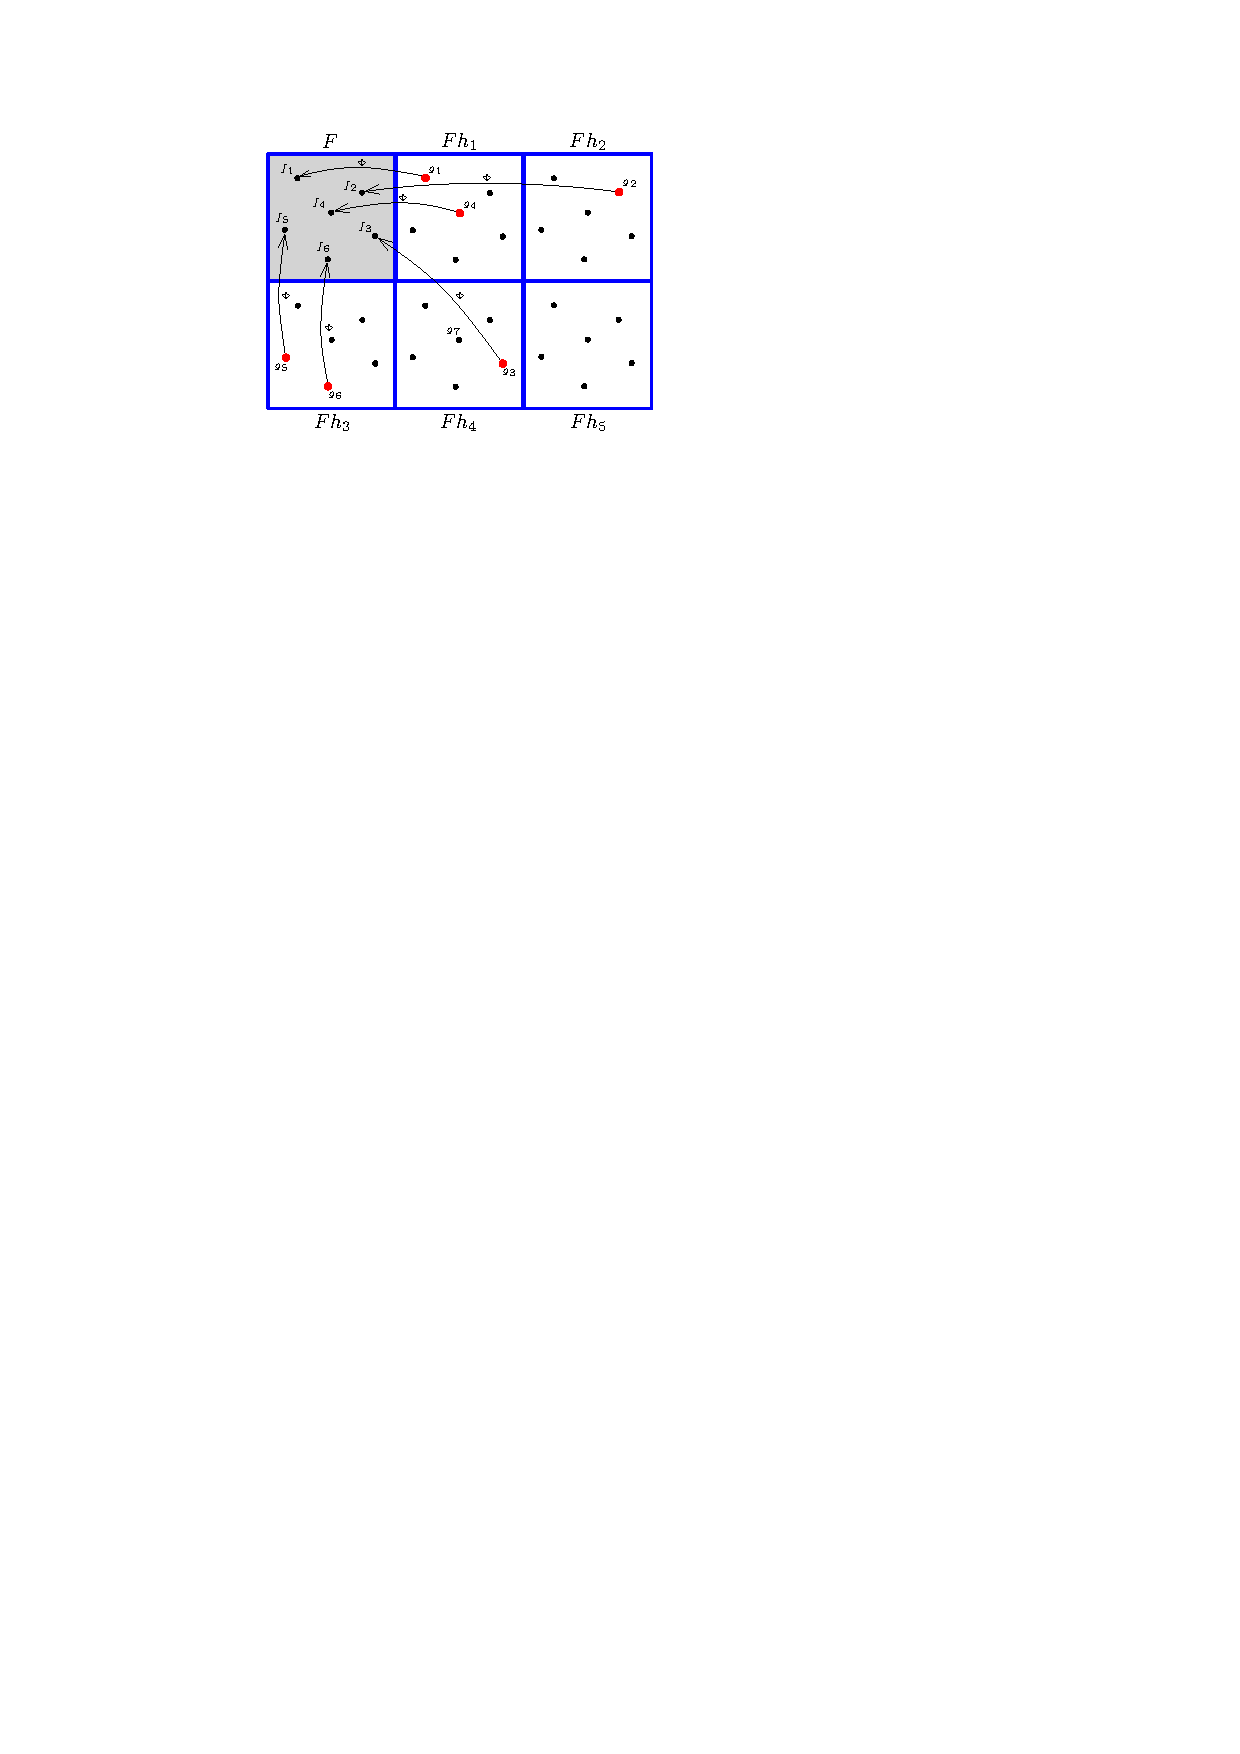
\includegraphics[scale=1.5]{../Graphics/obrazek_bijekcja}
\caption{We can see a sample set $F=\{f_1,\ldots,f_6\}$ and its shifts by some elements $h_1,\ldots, h_5\in H$. An element $g\in G\setminus H$ gives us a set $Fg=\{g_1,\ldots,g_6\}$ (marked in red). Arrows show how the map $\Phi$ acts on elements of $Fg$. Hence for instance, we have  $\Phi(g_1) = g_1h_1^{-1} = f_1$ and $\Phi(g_3) = g_3h_4^{-1} = f_3$. 
}\label{fig:bijekcja}
\end{figure}

\begin{proof}[Proof of Lemma \ref{lem:bijekcja_kafelkow}]
Let $f_1,f_2\in F$ and assume that $\Phi(f_1g)=\Phi(f_2g).$
Then there exist $h_1, h_2\in H$ such that $f_1gh_1^{-1},\,f_2gh_2^{-1}\in F$ and 
\[
f_1gh_1^{-1}=f_2gh_2^{-1}.
\]
This implies that
\[
f_1=f_2gh_2^{-1}h_1g^{-1}.
\]
Clearly, $gh_2^{-1}h_1g^{-1}\in H$ since $H$ is normal. But $F\cap Fh=\emptyset$ for every $h\in H\setminus\{e\}$. Therefore $gh_2^{-1}h_1g^{-1}=e$ and thus $f_1=f_2$.
\end{proof}


\noindent
Now the proof of Lemma \ref{lem:subordinate_periodic_entropy} is an almost straightforward consequence of the above considerations.

\begin{proof}[Proof of Lemma \ref{lem:subordinate_periodic_entropy}]
Since $z\in\{0,1\}^G$ is periodic, it satisfies $\htop(\closure{Gz})=0$ (Lemma \ref{lem:periodicEntropy}.), hence we can use Theorem \ref{thm:entropy-density}. Notice that it is enough to prove that 
\[
\frac{1}{|F_N|}\max\inbrace{\sum_{g\in F_N}w(g): w\in \mathcal B_{F_N}(\closure{Gz})} = \frac{1}{|F_N|}\sum_{g\in F_N} z(g) 
\]
because then, by periodicity of $z$, for every $n>N$ we obtain
\[
\frac{1}{|F_n|}\max\inbrace{\sum_{g\in F_n}w(g): w\in \mathcal B_{F_n}(\closure{Gz})} = \frac{1}{|F_N|}\sum_{g\in F_N} z(g) .
\]
Clearly we have
\[
\max\inbrace{\sum_{g\in F_N}w(g): w\in \mathcal B_{F_N}(\closure{Gz})} = \max\inbrace{\sum_{g\in F_Nh}z(g): h\in G}.
\]
Let $\Phi\colon G\to F_N$ satisfy $\Phi(g) = gh^{-1}$, where $h\in H_N$ is the unique element such that $g\in F_Nh$. 
By Lemma \ref{lem:bijekcja_kafelkow}. we know that $\Phi\restrict{F_Ng}$  is bijective for every $g\in G$ (see Figure \ref{fig:bijekcja}) which means that 
\[
\sum_{g\in F_Nh}z(g) =\sum_{g\in F_N} z(g) \quad \text{ for every } h\in G. \qedhere
\]

\end{proof}

